
The previous section explained how to cross-build OpenTURNS from Linux to target Windows.
This section gives hints in order to compile OpenTURNS natively with Microsoft Windows tools.
This port has started since OpenTURNS 1.4 and is still in an early stage, any help from developers
who are familiar with Windows environment will be greatly appreciated.

These instructions have been tested with Visual Studio 2010 on Windows 32 and 64 bits, but they should
work with more recent versions too.
Visual Studio Express Edition does not ship 64 bits compilers, but they can be installed
from Windows SDKs, instructions can be easily found online.  No Fortran compiler is required.

\subsection{Automatic compilation}

First of all, CMake must be installed, as well as C/C++ compilers.  We will describe below how
to use CMake with Visual Studio and Microsoft compilers, but CMake can also be used with other
build systems (like NMake, for instance) and other compilers, see CMake documentation for
further details.

The following programs are required in order to build OpenTURNS on Windows:
\begin{itemize}
\item Boost \url{https://www.boost.org/}
\item OpenBLAS \url{https://github.com/xianyi/OpenBLAS/} (or any other BLAS implementation)
\end{itemize}

The following programs are optional, and we will show how to embed them into OpenTURNS:
\begin{itemize}
\item hmat-oss \url{https://github.com/jeromerobert/hmat-oss/}
\item LibXML2 \url{http://www.xmlsoft.org/}
\item muParser \url{http://muparser.beltoforion.de/}
\item TBB \url{https://www.threadingbuildingblocks.org/}
\end{itemize}

Precompiled binaries for all these programs are available on \url{http://sourceforge.net/projects/openturns/files/openturns/openturns-x.y}.
If you want to recompile them from sources, you may also have to install
\begin{itemize}
\item Subversion \url{https://subversion.apache.org/}
\item Git \url{http://git-scm.com/}
\end{itemize}

The following programs are optional, and are currently not used by this native Windows port:
\begin{itemize}
\item R \url{http://www.r-project.org/}
\item Python \url{http://www.python.org/}
\end{itemize}
Some OpenTURNS components will thus not be available.  If R is installed on your computer, you should edit \texttt{openturns.conf} and set
\texttt{R-executable-command} resource in order to let OpenTURNS use it.  On the other hand, as OpenTURNS is built without Python bindings,
Python scripts cannot be used afterwards.

\subsubsection{Installation layout}

In this tutorial, OpenTURNS dependencies are installed by following the layout shown in figure~\ref{fig:win-inst-layout}.
Below the top-level directory are four configurations (Debug and Release for Windows 32 bits or 64 bits).  Of course,
if you are only interested by a single configuration, there is no need to create others.  Each configuration contains
subdirectories for Boost, hmat-oss, LibXML2, muParser, OpenBLAS and TBB programs.  Each project contains one or several
directories: \texttt{bin} for DLLs, \texttt{include} for header files, and \texttt{lib} for static libraries.

\begin{figure}[p]
\begin{center}
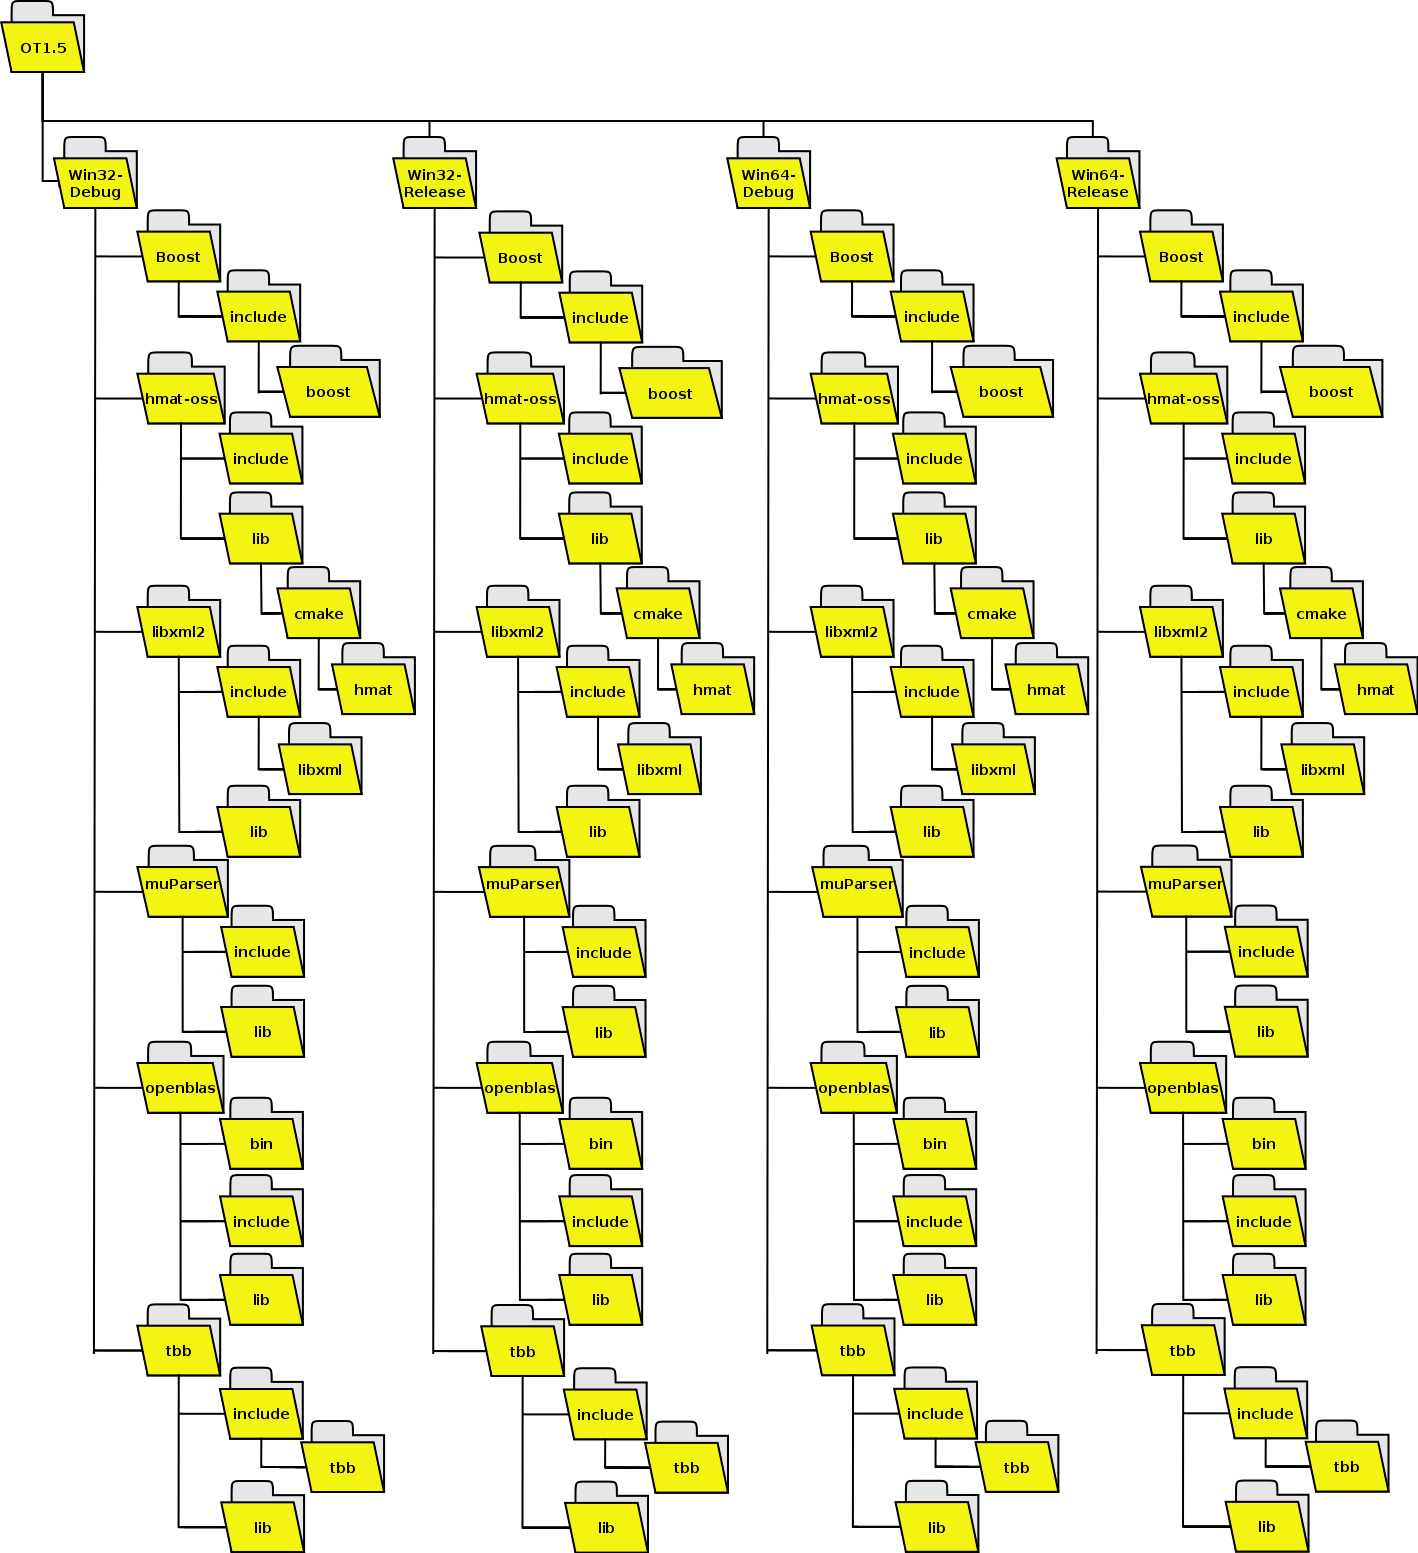
\includegraphics[scale=0.33]{Figures/win_native/win-inst-layout.png}
\caption{Windows installation layout}\label{fig:win-inst-layout}
\end{center}
\end{figure}

For convenience, all libraries will be compiled as static libraries, except OpenBLAS.

\subsubsection{Build and install OpenBLAS and TBB}

For different reasons, OpenBLAS and TBB cannot be compiled along with other dependencies.  As explained on
their site, OpenBLAS is currently only supported on Windows with Mingw compiler.  But binaries can be
used with Visual Studio, this is what we will do.  Thus go to
\url{http://sourceforge.net/projects/openblas/files/} and download Windows binaries, for instance
\url{OpenBLAS-v0.2.13-Win32.zip} for Windows 32 bits, and \url{OpenBLAS-v0.2.13-Win64-int32.zip}

Unzip these archives, and copy files to our installation folder:
\begin{itemize}
\item \verb+OpenBLAS-x.y-Win32\bin\libopenblas.dll+ into \verb+Win32-Release\openblas\bin\+ and\\
      \verb+Win32-Debug\openblas\bin\+
\item \verb+OpenBLAS-x.y-Win32\lib\libopenblas.dll.a+ into \verb+Win32-Release\openblas\lib\+ and\\
      \verb+Win32-Debug\openblas\lib\+
\item \verb+OpenBLAS-x.y-Win32\include+ into \verb+Win32-Release\openblas\+ and\\
      \verb+Win32-Debug\openblas\+
\item \verb+OpenBLAS-x.y-Win64-int32\bin\libopenblas.dll+ into \verb+Win64-Release\openblas\bin\+ and\\
      \verb+Win64-Debug\openblas\bin\+
\item \verb+OpenBLAS-x.y-Win64-int32\lib\libopenblas.dll.a+ into \verb+Win64-Release\openblas\lib\+ and\\
      \verb+Win64-Debug\openblas\lib\+
\item \verb+OpenBLAS-x.y-Win64-int32\include+ into \verb+Win64-Release\openblas\+ and\\
      \verb+Win64-Debug\openblas\+
\end{itemize}

Note that DLLs have been compiled with Mingw, and require some Mingw runtime libraries.  They can be found in
\url{http://sourceforge.net/projects/openblas/files/v0.2.12/mingw32_dll.zip} and
\url{http://sourceforge.net/projects/openblas/files/v0.2.12/mingw64_dll.zip}.
They are:
\begin{itemize}
\item \verb+libgcc_s_sjlj-1.dll+, \verb+libgfortran-3.dll+ and \verb+libquadmath-0.dll+ for Win32
\item \verb+libgcc_s_seh-1.dll+, \verb+libgfortran-3.dll+ and \verb+libquadmath-0.dll+ for Win64
\end{itemize}

TBB comes with its own Visual Studio 2010 configuration file, but we did not find how to integrate it into the build system described
below.  Thus the easiest solution is to:
\begin{enumerate}
\item Download TBB sources from \url{https://www.threadingbuildingblocks.org/download}
\item Unpack it.
\item Launch \verb+build\vs2010\makefile.sln+
\item Select \texttt{Win32} or \texttt{x64} architecture, and \texttt{Release} or \texttt{Debug} configuration (not \texttt{Release-MT} or \texttt{Debug-MT}, unless you know what you are doing).
\item If you want to build a static library, edit Properties, tab Configuration Properties, General, Configuration Type, as shown in figure~\ref{fig:vs-tbb-static}
\item Build project.
\item Copy resulting libraries into installation folder:
  \begin{itemize}
  \item \verb+build\vs2010\ia32\Debug\tbb_debug.lib+ into \verb+Win32-Debug\tbb\lib\+
  \item \verb+build\vs2010\ia32\Release\tbb.lib+ into \verb+Win32-Release\tbb\lib\+
  \item \verb+build\vs2010\intel64\Debug\tbb_debug.lib+ into \verb+Win64-Debug\tbb\lib\+
  \item \verb+build\vs2010\intel64\Release\tbb.lib+ into \verb+Win64-Release\tbb\lib\+
  \end{itemize}
\item Copy \verb+include\tbb+ folder into installation folders:
\verb+Win32-Debug\tbb\include+,\\
\verb+Win32-Release\tbb\include+,
\verb+Win64-Debug\tbb\include+
and \verb+Win64-Release\tbb\include+.
\end{enumerate}

\begin{figure}[htb]
\begin{center}
  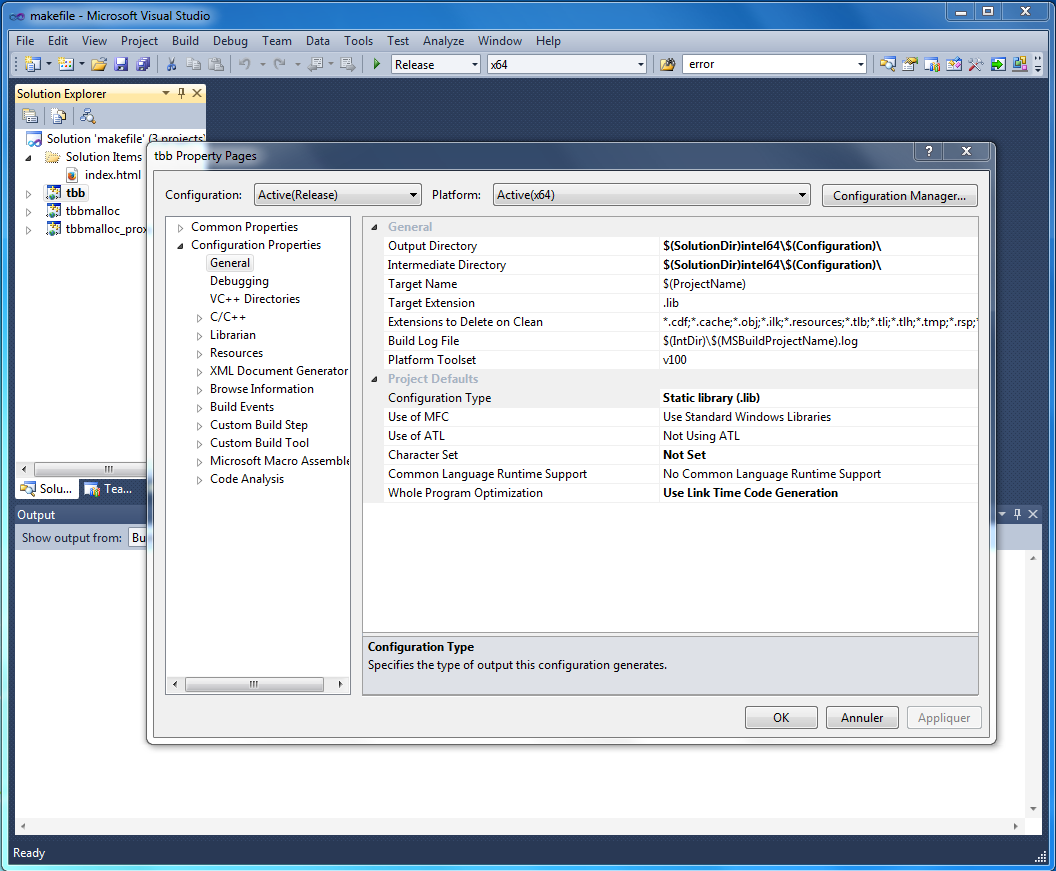
\includegraphics[scale=0.5]{Figures/win_native/vs-tbb-static.png}
\end{center}
\caption{Visual Studio settings to build tbb as a static library}
\label{fig:vs-tbb-static}
\end{figure}

\subsubsection{Build and install OpenTURNS}

OpenBLAS and TBB are low level libraries. Other libraries use STL, and care must be taken to avoid mismatch between runtime
libraries.  To this end, we decided to use a so called \emph{SuperBuild} approach with CMake.  We defined a metaproject
which drives compilation of those dependencies, and also of OpenTURNS itself.
Clone git repository \url{https://bitbucket.org/dbarbier/ot-superbuild} (or download an archive from this URL), launch
\texttt{cmake-gui} program, and follow the following steps:
\begin{enumerate}

\item Launch \texttt{cmake-gui}, and select source and build directories
\begin{center}
  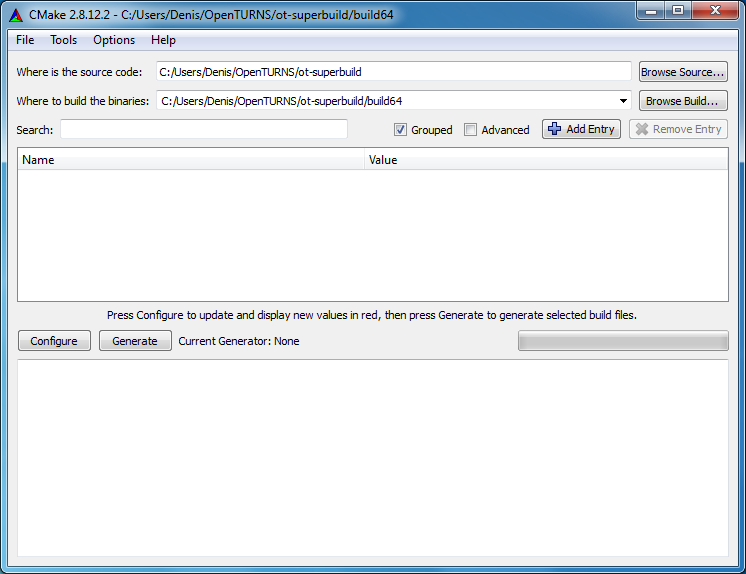
\includegraphics[scale=0.5]{Figures/win_native/cmake-gui-start.png}
\end{center}

\item Click on \textsf{Configure} button.  Select a generator (either Visual Studio 10 or Visual Studio 10 Win64) and compiler
\begin{center}
  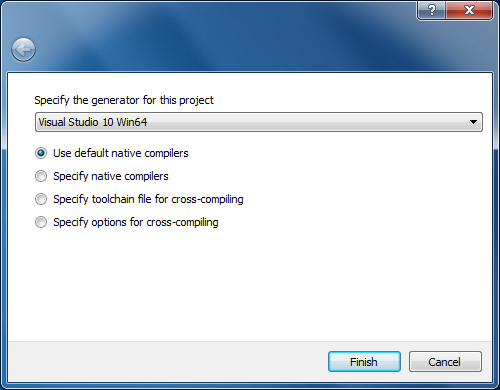
\includegraphics[scale=0.5]{Figures/win_native/cmake-gui-compiler.png}
\end{center}

\item For Win64, CMake may give an error about missing 64-bit tools, as in snapshot below.
Visual Studio Express Edition does not embed 64-bit compilers, and CMake thus checks whether
we are using Express Edition or not.
\begin{center}
  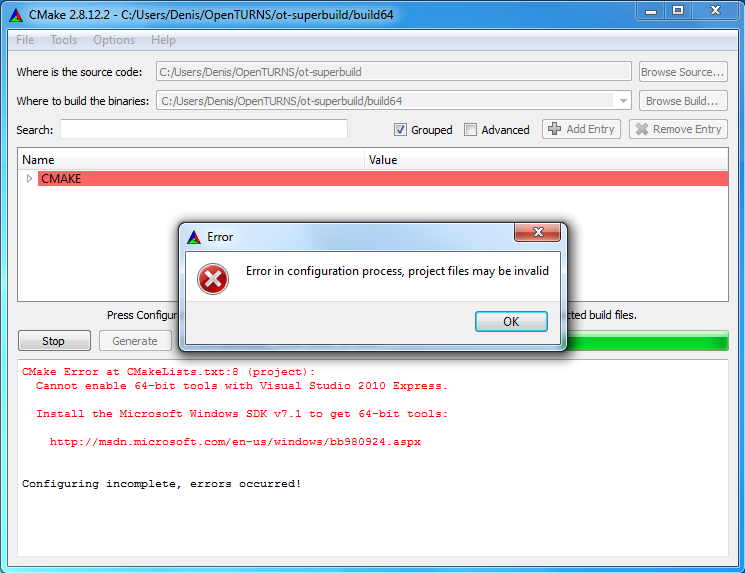
\includegraphics[scale=0.5]{Figures/win_native/cmake-gui-error.png}
\end{center}

It seems that this detection is sometimes buggy; if you know that 64-bit compilers are available,
you can workaround this automatic detection by clicking on \textsf{Add Entry} button, adding a
\texttt{CMAKE\_GENERATOR\_TOOLSET} variable, of type \texttt{STRING}, and value \texttt{v100}.
\begin{center}
  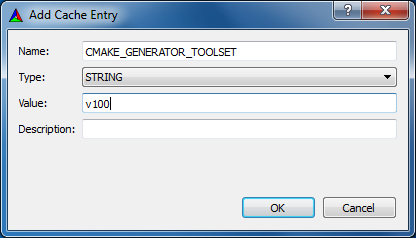
\includegraphics[scale=0.5]{Figures/win_native/cmake-gui-toolset.png}
\end{center}

\item Click on \textsf{Configure} button again, everything should work fine now, and output window should
display \texttt{Configuring done}.

\item Now that CMake has checked that our compiler is working fine, we can tell it where to find OpenBLAS and TBB.
Set \texttt{OPENBLAS\_INCLUDE\_DIR}, \texttt{OPENBLAS\_LIBRARY}, \texttt{TBB\_INCLUDE\_DIR} and
\texttt{TBB\_LIBRARY} variables, as shown below:
\begin{center}
  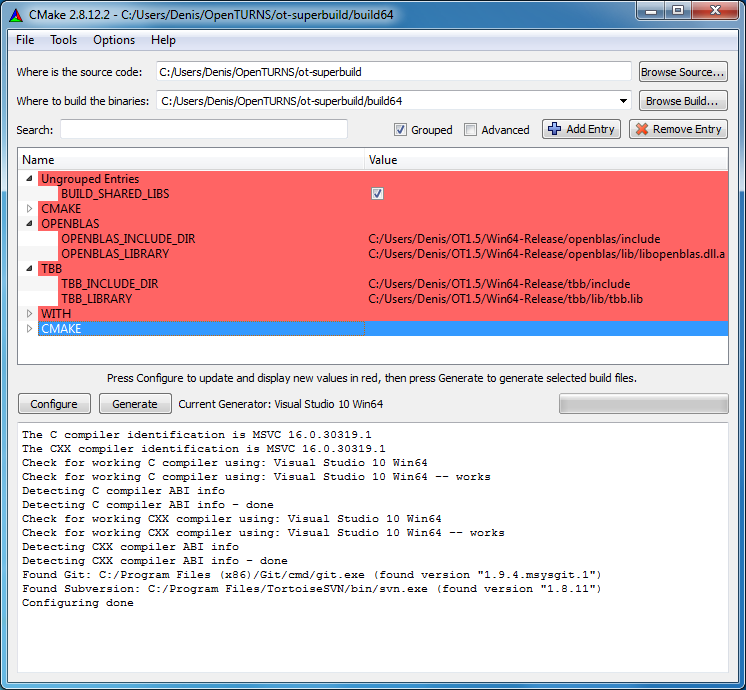
\includegraphics[scale=0.5]{Figures/win_native/cmake-gui-superbuild.png}
\end{center}
and click on \textsf{Configure} button.

\item If everything went fine, click on \textsf{Generate} button.  This generates Visual Studio solution files in the specified
build directory, and you can now close \texttt{cmake-gui} window.

\item Launch \texttt{openturns-superbuild} solution file.
\begin{center}
  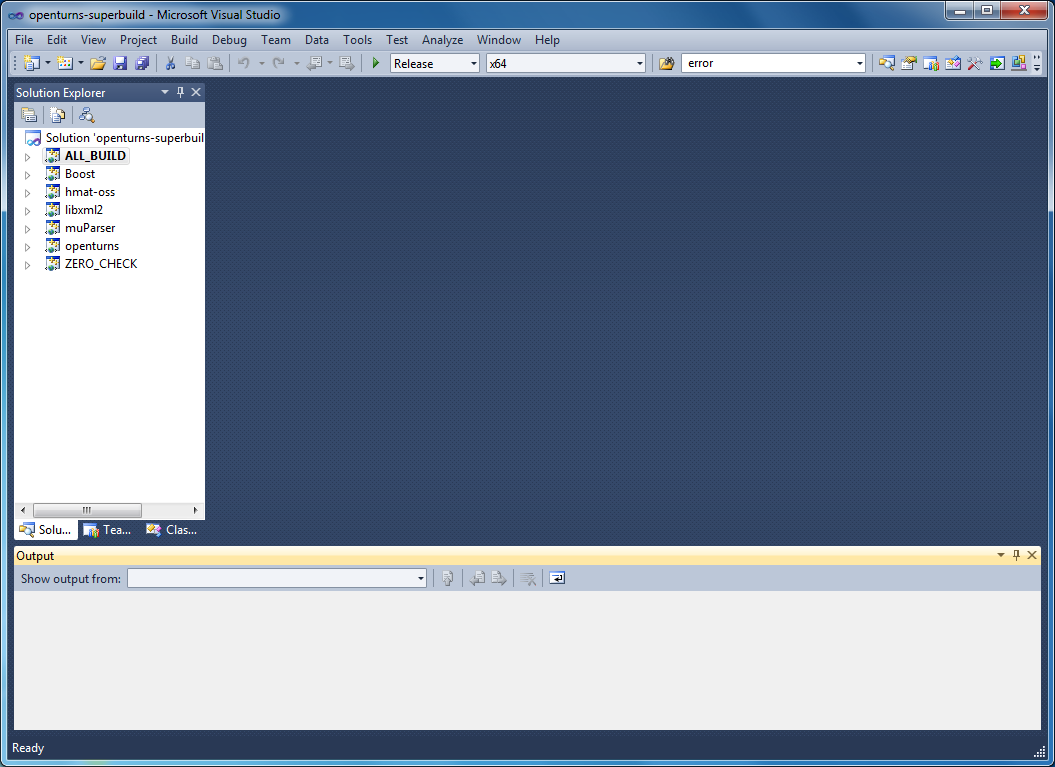
\includegraphics[scale=0.5]{Figures/win_native/vs-superbuild.png}
\end{center}
Select \texttt{Release} or \texttt{Debug} configuration (it must match TBB configuration), and build solution file.
This will download sources (a working Internet connection is thus required), unpack and build them.
It can take a long time on a slow machine, or with a slow Internet connection, since some downloaded sources are large.
\item Copy \verb+build64\ExternalProjects\Install\*+ directories into installation prefix (\verb+OT1.5\Win64-Release\+, or \verb+Win32-Release+,
etc)
\end{enumerate}

\subsection{Manual compilation}

If you want to modify settings, the simplest solution is to proceed as in previous section, and modify Visual Studio settings afterwards.
Dependencies are downloaded, built and installed into an \verb+ExternalProjects+ subdirectory of build directory, ie
\verb+build64\ExternalProjects+ in our example.  This directory contains the following folders:
\begin{itemize}
\item \texttt{Build}: contains generated Visual Studio projects, and files generated during builds
\item \texttt{Download}: contains project archives
\item \texttt{Install}: after build, each project installs resulting files (header files and libraries) there
\item \texttt{Source}: unpacked source files
\item \texttt{Stamp}: keeps track of already processed steps
\item \texttt{tmp}
\end{itemize}
Each directory in turn contains one directory per project.  Thus if one wants to modify some settings when compiling OpenTURNS,
one has to go to \verb+build64\ExternalProjects\Build\openturns\+ directory and launch the Visual Studio solution file found there,
in this case \texttt{OpenTURNS.sln}.  For instance, one can build OpenTURNS tests from this solution file.
Beware to always check that active configuration is the desired one.

\subsection{Unresolved problems}
\paragraph{Python bindings are not generated}

After installing SWIG and Python binaries, we had been able to generate Python modules without trouble, but Python could not load
those modules.  It seems that the same version of Visual Studio must be used to compile Python and modules, but we could only find
Python binaries built with Visual Studio 9.  The solution is to build Python from sources, but this had not been tested yet.

\paragraph{Tests are not run}

Tests can be compiled but not launched from Visual Studio, because they are run via shell commands, and also because tests executable are
generated in a subdirectory.  It is possible to work around those limitations and run tests, but this is currently not automated.

\subsection{Troubleshooting}
\begin{itemize}
\item It is possible to build multiple configurations with Visual Studio solution files, but this is currently not supported by
our \texttt{CMakeLists.txt} files; thus one must launch \texttt{cmake-gui}, adapt variables (for instance paths to OpenBLAS
and TBB libraries must be modified for each configuration) and press \textsf{Configure} and \textsf{Generate} buttons.
\item No OpenBLAS library in \texttt{Debug} mode is provided, but the one from \texttt{Release} mode works also in \texttt{Debug}
mode.  On the other hand, OpenTURNS and TBB configurations must match, it is not possible to link OpenTURNS in \texttt{Debug} mode
against TBB in \texttt{Release} mode, or vice-versa.
\item Boost contains files with very long filenames, which causes trouble on NTFS.  If you have already built Boost and want to
build it again, Visual Studio may complain that it encountered an error when building it again.  In that case, launch file
explorer and remove Boost directory, then press again \textsf{Generate} button of CMake (because some of its generated files had
been removed too), it should now build fine.
\end{itemize}
